\documentclass[12pt]{exam}
\usepackage{amsthm}
\usepackage{libertine}
\usepackage[utf8]{inputenc}
\usepackage[margin=1in]{geometry}
\usepackage{amsmath,amssymb}
\usepackage{multicol}
\usepackage[shortlabels]{enumitem}
\usepackage{siunitx}
\usepackage{booktabs}
\usepackage{graphicx}
\usepackage{pgfplots}
\usepackage{listings}
\usepackage{tikz}



\pgfplotsset{width=10cm,compat=1.9}
\usepgfplotslibrary{external}
%\tikzexternalize

\newcommand{\class}{Math 101-002} % This is the name of the course 
\newcommand{\examnum}{Exam 2 Makeup} % This is the name of the assignment
\newcommand{\examdate}{March 26} % This is the due date





\begin{document}
\pagestyle{plain}
\thispagestyle{empty}

\noindent
\textbf{\class}\\
\textbf{\examnum}, \textbf{\examdate} \\

% Name \hfill CSU ID \# \hspace{2.25in}

%\vspace{10 pt}

\setlength{\tabcolsep}{3.5cm} % Default value: 6pt
\renewcommand{\arraystretch}{1.5}
\setlength\extrarowheight{1cm}
\begin{tabular}{ |c|c| } 
 \hline
 Name   & CSU ID \#  \\ 
 \hline
\end{tabular}
% ---
\vspace{10pt}

Be sure to read each question fully and carefully. Multiple choice answer bubbles must be fully filled in.  There is space to the right of each multiple choice question to show work, if your work is correct you can get points even with an incorrect multiple choice answer.  


\iffalse

    \foreach \s in {1,...,5}{
          \choice $P_\s$ has no power 
     }%;
\fi


\begin{enumerate} 

\item For questions \ref{firstQnSec1} through \ref{lastQnSec1} consider the following weighted graph G:\par

\begin{figure}[h!]
    \centering


    \tikzset{every picture/.style={line width=0.75pt}} %set default line width to 0.75pt        

    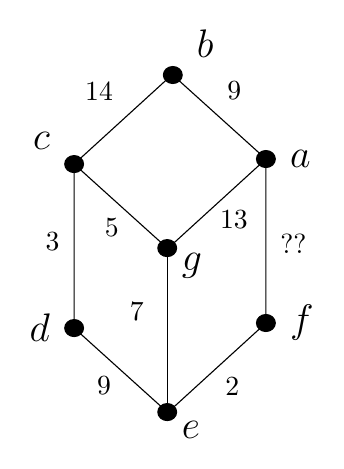
\begin{tikzpicture}[x=0.75pt,y=0.75pt,yscale=-1,xscale=1]
    %uncomment if require: \path (0,244); %set diagram left start at 0, and has height of 244
    
    %Shape: Cube [id:dp6646435130858394] 
    \draw   (39.45,81.85) -- (86.73,38.72) -- (131.84,79.43) -- (131.84,158.44) -- (84.55,201.57) -- (39.45,160.85) -- cycle ; \draw   (131.84,79.43) -- (84.55,122.56) -- (39.45,81.85) ; \draw   (84.55,122.56) -- (84.55,201.57) ;
    %Shape: Ellipse [id:dp7053935929182301] 
    \draw  [fill={rgb, 255:red, 0; green, 0; blue, 0 }  ,fill opacity=1 ] (82.46,38.95) .. controls (82.46,36.69) and (84.49,34.86) .. (86.99,34.86) .. controls (89.49,34.86) and (91.52,36.69) .. (91.52,38.95) .. controls (91.52,41.2) and (89.49,43.03) .. (86.99,43.03) .. controls (84.49,43.03) and (82.46,41.2) .. (82.46,38.95) -- cycle ;
    %Shape: Ellipse [id:dp3846430227043952] 
    \draw  [fill={rgb, 255:red, 0; green, 0; blue, 0 }  ,fill opacity=1 ] (127.31,79.42) .. controls (127.31,77.17) and (129.34,75.34) .. (131.84,75.34) .. controls (134.34,75.34) and (136.37,77.17) .. (136.37,79.42) .. controls (136.37,81.68) and (134.34,83.51) .. (131.84,83.51) .. controls (129.34,83.51) and (127.31,81.68) .. (127.31,79.42) -- cycle ;
    %Shape: Ellipse [id:dp3122259521210028] 
    \draw  [fill={rgb, 255:red, 0; green, 0; blue, 0 }  ,fill opacity=1 ] (79.77,122.33) .. controls (79.77,120.07) and (81.79,118.25) .. (84.29,118.25) .. controls (86.8,118.25) and (88.82,120.07) .. (88.82,122.33) .. controls (88.82,124.59) and (86.8,126.42) .. (84.29,126.42) .. controls (81.79,126.42) and (79.77,124.59) .. (79.77,122.33) -- cycle ;
    %Shape: Ellipse [id:dp5568900450079106] 
    \draw  [fill={rgb, 255:red, 0; green, 0; blue, 0 }  ,fill opacity=1 ] (34.92,81.86) .. controls (34.92,79.6) and (36.95,77.77) .. (39.45,77.77) .. controls (41.95,77.77) and (43.97,79.6) .. (43.97,81.86) .. controls (43.97,84.11) and (41.95,85.94) .. (39.45,85.94) .. controls (36.95,85.94) and (34.92,84.11) .. (34.92,81.86) -- cycle ;
    %Shape: Ellipse [id:dp5276475452889409] 
    \draw  [fill={rgb, 255:red, 0; green, 0; blue, 0 }  ,fill opacity=1 ] (34.92,160.86) .. controls (34.92,158.61) and (36.95,156.78) .. (39.45,156.78) .. controls (41.95,156.78) and (43.97,158.61) .. (43.97,160.86) .. controls (43.97,163.12) and (41.95,164.95) .. (39.45,164.95) .. controls (36.95,164.95) and (34.92,163.12) .. (34.92,160.86) -- cycle ;
    %Shape: Ellipse [id:dp01895932765963071] 
    \draw  [fill={rgb, 255:red, 0; green, 0; blue, 0 }  ,fill opacity=1 ] (79.77,201.34) .. controls (79.77,199.08) and (81.79,197.25) .. (84.29,197.25) .. controls (86.8,197.25) and (88.82,199.08) .. (88.82,201.34) .. controls (88.82,203.6) and (86.8,205.43) .. (84.29,205.43) .. controls (81.79,205.43) and (79.77,203.6) .. (79.77,201.34) -- cycle ;
    %Shape: Ellipse [id:dp8485087793178528] 
    \draw  [fill={rgb, 255:red, 0; green, 0; blue, 0 }  ,fill opacity=1 ] (127.31,158.43) .. controls (127.31,156.17) and (129.34,154.34) .. (131.84,154.34) .. controls (134.34,154.34) and (136.37,156.17) .. (136.37,158.43) .. controls (136.37,160.69) and (134.34,162.52) .. (131.84,162.52) .. controls (129.34,162.52) and (127.31,160.69) .. (127.31,158.43) -- cycle ;
    
    % Text Node
    \draw (142.19,79.42) node [anchor=west] [inner sep=0.75pt]  [font=\Large]  {$a$};
    % Text Node
    \draw (97.34,31.74) node [anchor=south west] [inner sep=0.75pt]  [font=\Large]  {$b$};
    % Text Node
    \draw (29.1,76.02) node [anchor=south east] [inner sep=0.75pt]  [font=\Large]  {$c$};
    % Text Node
    \draw (29.1,160.86) node [anchor=east] [inner sep=0.75pt]  [font=\Large]  {$d$};
    % Text Node
    \draw (90.12,204.46) node [anchor=north west][inner sep=0.75pt]  [font=\Large]  {$e$};
    % Text Node
    \draw (142.19,158.43) node [anchor=west] [inner sep=0.75pt]  [font=\Large]  {$f$};
    % Text Node
    \draw (90.12,123.54) node [anchor=north west][inner sep=0.75pt]  [font=\Large]  {$g$};
    % Text Node
    \draw (112,40.9) node [anchor=north west][inner sep=0.75pt]    {$9$};
    % Text Node
    \draw (108.5,102.9) node [anchor=north west][inner sep=0.75pt]    {$13$};
    % Text Node
    \draw (137.5,114.4) node [anchor=north west][inner sep=0.75pt]    {$??$};
    % Text Node
    \draw (58.44,182.9) node [anchor=north east] [inner sep=0.75pt]    {$9$};
    % Text Node
    \draw (24.5,113.4) node [anchor=north west][inner sep=0.75pt]    {$3$};
    % Text Node
    \draw (43.5,41.4) node [anchor=north west][inner sep=0.75pt]    {$14$};
    % Text Node
    \draw (111,183.4) node [anchor=north west][inner sep=0.75pt]    {$2$};
    % Text Node
    \draw (53,106.9) node [anchor=north west][inner sep=0.75pt]    {$5$};
    % Text Node
    \draw (65,147.4) node [anchor=north west][inner sep=0.75pt]    {$7$};
    
    
    \end{tikzpicture}
    

    
\end{figure}

\begin{enumerate}
    \item \label{firstQnSec1} Write down the list of vertices of the graph $G$: (2 points)
    \vspace{0.5em}
    $$V=\left\lbrace\underline{\phantom{ans}},\underline{\phantom{ans}},\underline{\phantom{ans}},\underline{\phantom{ans}},\underline{\phantom{ans}},\underline{\phantom{ans}},\underline{\phantom{ans}}\right\rbrace.$$
    \vfill
    \item Write down the list of edges of the graph $G$: (2 points)
    \vspace{0.5em}
    $$E=\left\lbrace\underline{\phantom{ans}},\underline{\phantom{ans}},\underline{\phantom{ans}},\underline{\phantom{ans}},\underline{\phantom{ans}},\underline{\phantom{ans}},\underline{\phantom{ans}},\underline{\phantom{ans}},\underline{\phantom{ans}}\right\rbrace.$$
    \vfill
    \item Out of the following, which is \textbf{NOT} an edge in the graph? (2 points)
    \begin{checkboxes}
        \choice $bg$
        \choice $cd$
        \choice $eg$
        \choice $af$
    \end{checkboxes}
    \vfill
    \item How many vertices does this graph have? (2 points)
    \begin{checkboxes}
        \choice 3
        \choice 6
        \choice 7
        \choice 8
    \end{checkboxes}
    \vfill
    \newpage
    \item The degree of the vertex $a$ is: (2 points)
    \vspace{0.5em}
    $$\deg(a)=\underline{\phantom{ans}}.$$
    \vfill
    \item The degree of the vertex $e$ is: (2 points)
    \vspace{0.5em}
    $$\deg(e)=\underline{\phantom{ans}}.$$
    \vfill
    \item A path of length $5$ from $c$ to $g$ passing through $a$ is: (2 points)
    \begin{checkboxes}
        \choice $cg$
        \choice $cb,ba,af,fe,ed$
        \choice $cd,de,ef,fa,ag$
        \choice $ga,ab,ba,ag,gc$
    \end{checkboxes}
    \vfill
    \item For the weight of the previous path to be $35$, the missing weight should be: (2 points)
    \vspace{0.5em}
    $$\text{weight}=\underline{\phantom{ans}}.$$
    \vfill
    \item Does this graph $G$ have cut-edges (bridges)? (2 points)
    \begin{checkboxes}
        \choice Yes.
        \choice No.
    \end{checkboxes}
    \vfill
    \item State whether this graph has an Euler walk. If it does, write it down, if not state why it doesn't. (2 points)
    \vspace{8em}
    \vfill
    \item State whether this graph has an Hamilton walk. If it does, write it down, if not state why it doesn't. (2 points)
    \vspace{8em}
    \vfill
    \newpage
    \item The graph $G$ doesn't have an Euler circuit, Eulerize it by adding edges: (2 points)
    \begin{figure}[h]
        \centering
        \tikzset{every picture/.style={line width=0.75pt}} %set default line width to 0.75pt        
    
        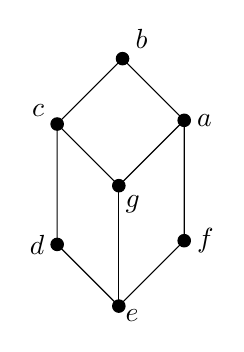
\begin{tikzpicture}[x=0.75pt,y=0.75pt,yscale=-1,xscale=1]
        %uncomment if require: \path (0,300); %set diagram left start at 0, and has height of 300
        
        %Shape: Cube [id:dp6646435130858394] 
        \draw   (30.79,59.04) -- (62.29,27.54) -- (92,57.25) -- (92,115.25) -- (60.5,146.75) -- (30.79,117.04) -- cycle ; \draw   (92,57.25) -- (60.5,88.75) -- (30.79,59.04) ; \draw   (60.5,88.75) -- (60.5,146.75) ;
        %Shape: Circle [id:dp7053935929182301] 
        \draw  [fill={rgb, 255:red, 0; green, 0; blue, 0 }  ,fill opacity=1 ] (59.29,27.54) .. controls (59.29,25.88) and (60.63,24.54) .. (62.29,24.54) .. controls (63.94,24.54) and (65.29,25.88) .. (65.29,27.54) .. controls (65.29,29.19) and (63.94,30.54) .. (62.29,30.54) .. controls (60.63,30.54) and (59.29,29.19) .. (59.29,27.54) -- cycle ;
        %Shape: Circle [id:dp3846430227043952] 
        \draw  [fill={rgb, 255:red, 0; green, 0; blue, 0 }  ,fill opacity=1 ] (89,57.25) .. controls (89,55.59) and (90.34,54.25) .. (92,54.25) .. controls (93.66,54.25) and (95,55.59) .. (95,57.25) .. controls (95,58.91) and (93.66,60.25) .. (92,60.25) .. controls (90.34,60.25) and (89,58.91) .. (89,57.25) -- cycle ;
        %Shape: Circle [id:dp3122259521210028] 
        \draw  [fill={rgb, 255:red, 0; green, 0; blue, 0 }  ,fill opacity=1 ] (57.5,88.75) .. controls (57.5,87.09) and (58.84,85.75) .. (60.5,85.75) .. controls (62.16,85.75) and (63.5,87.09) .. (63.5,88.75) .. controls (63.5,90.41) and (62.16,91.75) .. (60.5,91.75) .. controls (58.84,91.75) and (57.5,90.41) .. (57.5,88.75) -- cycle ;
        %Shape: Circle [id:dp5568900450079106] 
        \draw  [fill={rgb, 255:red, 0; green, 0; blue, 0 }  ,fill opacity=1 ] (27.79,59.04) .. controls (27.79,57.38) and (29.13,56.04) .. (30.79,56.04) .. controls (32.44,56.04) and (33.79,57.38) .. (33.79,59.04) .. controls (33.79,60.69) and (32.44,62.04) .. (30.79,62.04) .. controls (29.13,62.04) and (27.79,60.69) .. (27.79,59.04) -- cycle ;
        %Shape: Circle [id:dp5276475452889409] 
        \draw  [fill={rgb, 255:red, 0; green, 0; blue, 0 }  ,fill opacity=1 ] (27.79,117.04) .. controls (27.79,115.38) and (29.13,114.04) .. (30.79,114.04) .. controls (32.44,114.04) and (33.79,115.38) .. (33.79,117.04) .. controls (33.79,118.69) and (32.44,120.04) .. (30.79,120.04) .. controls (29.13,120.04) and (27.79,118.69) .. (27.79,117.04) -- cycle ;
        %Shape: Circle [id:dp01895932765963071] 
        \draw  [fill={rgb, 255:red, 0; green, 0; blue, 0 }  ,fill opacity=1 ] (57.5,146.75) .. controls (57.5,145.09) and (58.84,143.75) .. (60.5,143.75) .. controls (62.16,143.75) and (63.5,145.09) .. (63.5,146.75) .. controls (63.5,148.41) and (62.16,149.75) .. (60.5,149.75) .. controls (58.84,149.75) and (57.5,148.41) .. (57.5,146.75) -- cycle ;
        %Shape: Circle [id:dp8485087793178528] 
        \draw  [fill={rgb, 255:red, 0; green, 0; blue, 0 }  ,fill opacity=1 ] (89,115.25) .. controls (89,113.59) and (90.34,112.25) .. (92,112.25) .. controls (93.66,112.25) and (95,113.59) .. (95,115.25) .. controls (95,116.91) and (93.66,118.25) .. (92,118.25) .. controls (90.34,118.25) and (89,116.91) .. (89,115.25) -- cycle ;
        
        % Text Node
        \draw (97,57.25) node [anchor=west] [inner sep=0.75pt]    {$a$};
        % Text Node
        \draw (67.29,24.14) node [anchor=south west] [inner sep=0.75pt]    {$b$};
        % Text Node
        \draw (25.79,56.64) node [anchor=south east] [inner sep=0.75pt]    {$c$};
        % Text Node
        \draw (25.79,117.04) node [anchor=east] [inner sep=0.75pt]    {$d$};
        % Text Node
        \draw (62.5,147.15) node [anchor=north west][inner sep=0.75pt]    {$e$};
        % Text Node
        \draw (97,115.25) node [anchor=west] [inner sep=0.75pt]    {$f$};
        % Text Node
        \draw (62.5,92.15) node [anchor=north west][inner sep=0.75pt]    {$g$};
        
        
        \end{tikzpicture}
        
    \end{figure}
    \vfill 
    \item Assume you start traveling the graph $G$ at the vertex $f$. If you are applying the Nearest-Neighbor algorithm and you traveled to the vertex $a$ instead of $e$, then the weight of $af$ was: (2 points)
    \begin{checkboxes}
        \choice 1
        \choice 2
        \choice 3
        \choice 4
    \end{checkboxes}
    \vfill
    \item When traveling the graph $G$, you arrived at the vertex $e$ from $f$. Following the Nearest-Neighbor algorithm, which vertex should you visit next? (2 points)
    \begin{checkboxes}
        \choice $a$
        \choice $b$
        \choice $d$
        \choice $g$
    \end{checkboxes}
    \vfill
    \item When applying the Cheapest-Link algorithm, suppose you have already picked the edges $ef$, $cd$, $cg$ and $eg$. Which edge should be picked next? (2 points)
    \begin{checkboxes}
        \choice $ab$
        \choice $bc$
        \choice $de$
        \choice $ef$
    \end{checkboxes}
    \vfill
    \item \label{lastQnSec1} Suppose you're applying Cheapest-Link algorithm to $G$. For $af$ to be $3^{\text{rd}}$ edge you pick, its weight should be: (2 points)
    \vspace{0.5em}
    $$\text{weight}(af)=\underline{\phantom{ans}}.$$
    \vfill
\end{enumerate}
\newpage
\item For questions \ref{firstQnSec2} through \ref{lastQnSec2} consider the information about the graph $G$ given by the following lists:
\begin{gather*}
    V=\left\lbrace a,b,c,d,e,f\right\rbrace,\\
    E=\left\lbrace ad,ae,bc,bd,cd,de,df,ea,ef\right\rbrace,\\
    W=\left\lbrace 7,6,8,9,5,6,4,10,7\right\rbrace.
\end{gather*}
The weights are ordered respecting the order of the edges.
\begin{enumerate}
\item \label{firstQnSec2} Fill in the weighted edges of the graph $G$ (Hint: Pay attention to the repeated edge): (4 points)
\begin{figure}[h!]
    \centering
   


    \tikzset{every picture/.style={line width=0.75pt}} %set default line width to 0.75pt        

    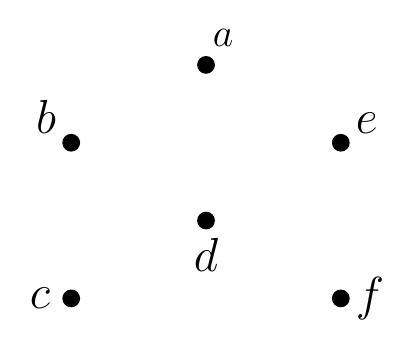
\begin{tikzpicture}[x=0.75pt,y=0.75pt,yscale=-1,xscale=1]
    %uncomment if require: \path (0,300); %set diagram left start at 0, and has height of 300
    
    %Shape: Circle [id:dp24175619248880365] 
    \draw  [fill={rgb, 255:red, 0; green, 0; blue, 0 }  ,fill opacity=1 ] (33.5,99.95) .. controls (33.5,97.74) and (35.29,95.95) .. (37.5,95.95) .. controls (39.71,95.95) and (41.5,97.74) .. (41.5,99.95) .. controls (41.5,102.16) and (39.71,103.95) .. (37.5,103.95) .. controls (35.29,103.95) and (33.5,102.16) .. (33.5,99.95) -- cycle ;
    %Shape: Circle [id:dp38562246159096747] 
    \draw  [fill={rgb, 255:red, 0; green, 0; blue, 0 }  ,fill opacity=1 ] (98.45,62.45) .. controls (98.45,60.24) and (100.24,58.45) .. (102.45,58.45) .. controls (104.66,58.45) and (106.45,60.24) .. (106.45,62.45) .. controls (106.45,64.66) and (104.66,66.45) .. (102.45,66.45) .. controls (100.24,66.45) and (98.45,64.66) .. (98.45,62.45) -- cycle ;
    %Shape: Circle [id:dp9956752087587961] 
    \draw  [fill={rgb, 255:red, 0; green, 0; blue, 0 }  ,fill opacity=1 ] (163.4,174.95) .. controls (163.4,172.74) and (165.19,170.95) .. (167.4,170.95) .. controls (169.61,170.95) and (171.4,172.74) .. (171.4,174.95) .. controls (171.4,177.16) and (169.61,178.95) .. (167.4,178.95) .. controls (165.19,178.95) and (163.4,177.16) .. (163.4,174.95) -- cycle ;
    %Shape: Circle [id:dp24033698556569782] 
    \draw  [fill={rgb, 255:red, 0; green, 0; blue, 0 }  ,fill opacity=1 ] (33.5,174.95) .. controls (33.5,172.74) and (35.29,170.95) .. (37.5,170.95) .. controls (39.71,170.95) and (41.5,172.74) .. (41.5,174.95) .. controls (41.5,177.16) and (39.71,178.95) .. (37.5,178.95) .. controls (35.29,178.95) and (33.5,177.16) .. (33.5,174.95) -- cycle ;
    %Shape: Circle [id:dp10560264310320788] 
    \draw  [fill={rgb, 255:red, 0; green, 0; blue, 0 }  ,fill opacity=1 ] (98.45,137.45) .. controls (98.45,135.24) and (100.24,133.45) .. (102.45,133.45) .. controls (104.66,133.45) and (106.45,135.24) .. (106.45,137.45) .. controls (106.45,139.66) and (104.66,141.45) .. (102.45,141.45) .. controls (100.24,141.45) and (98.45,139.66) .. (98.45,137.45) -- cycle ;
    %Shape: Circle [id:dp03400871765845248] 
    \draw  [fill={rgb, 255:red, 0; green, 0; blue, 0 }  ,fill opacity=1 ] (163.4,99.95) .. controls (163.4,97.74) and (165.19,95.95) .. (167.4,95.95) .. controls (169.61,95.95) and (171.4,97.74) .. (171.4,99.95) .. controls (171.4,102.16) and (169.61,103.95) .. (167.4,103.95) .. controls (165.19,103.95) and (163.4,102.16) .. (163.4,99.95) -- cycle ;
    
    % Text Node
    \draw (104.45,55.05) node [anchor=south west] [inner sep=0.75pt]  [font=\Large]  {$a$};
    % Text Node
    \draw (31.5,96.55) node [anchor=south east] [inner sep=0.75pt]  [font=\LARGE]  {$b$};
    % Text Node
    \draw (28.5,174.95) node [anchor=east] [inner sep=0.75pt]  [font=\LARGE]  {$c$};
    % Text Node
    \draw (102.45,144.85) node [anchor=north] [inner sep=0.75pt]  [font=\LARGE]  {$d$};
    % Text Node
    \draw (173.4,174.95) node [anchor=west] [inner sep=0.75pt]  [font=\LARGE]  {$f$};
    % Text Node
    \draw (173.4,96.55) node [anchor=south west] [inner sep=0.75pt]  [font=\LARGE]  {$e$};
    
    
    \end{tikzpicture}
\end{figure}
\vfill
\item List all the vertices adjacent to $d$: (2 points)
$$N(d)=\left\lbrace\underline{\phantom{ans}},\underline{\phantom{ans}},\underline{\phantom{ans}},\underline{\phantom{ans}},\underline{\phantom{ans}}\right\rbrace$$

\vfill
\item What are the degrees of the vertices $a$ and $f$? (4 points)
$$\deg(a)=\underline{\phantom{ans}}\quad\text{and}\quad\deg(f)=\underline{\phantom{ans}}.$$
\vfill
\item Find the sum of the degrees of all vertices: (2 points)
\begin{checkboxes}
    \choice 6
    \choice 9
    \choice 12
    \choice 18
\end{checkboxes}
\vfill
\item State whether this graph has an Euler walk. If it does, write it down, if not state why it doesn't. (2 points)
    \vspace{7em}
\vfill
\item The graph $G$ doesn't have an Euler circuit. Only one edge is needed to make it Eulerian. Which is that edge? (2 points)
  $$\text{missing edge}=\underline{\phantom{ans}}.$$
\vfill
\item Does this graph $G$ have cut-edges (bridges)? (2 points)
    \begin{checkboxes}
        \choice Yes.
        \choice No.
    \end{checkboxes}
    \vfill
\item What is the weight of the path $\left\lbrace bc,cd,df,fe\right\rbrace$? (2 points)
\begin{checkboxes}
    \choice 5
    \choice 8
    \choice 20
    \choice 24
\end{checkboxes}
\vfill
\item When traveling the graph $G$ starting at $e$, your Nearest-Neighbor algorithm took you to $a$ and then $d$. The next vertex you should visit is: (2 points)
\begin{checkboxes}
    \choice $b$
    \choice $c$
    \choice $e$
    \choice $f$
\end{checkboxes}
\vfill
\item The Nearest-Neighbor algorithm starting at the vertex $b$ produces a walk that ends at which vertex? (2 points)
\begin{checkboxes}
    \choice $a$
    \choice $b$
    \choice $d$
    \choice $f$
\end{checkboxes}
\vfill
\item \label{lastQnSec2} Which is the edge that you pick first in $G$ when applying the Cheapest-Link algorithm? (2 points)
$$1^{\text{st}}\text{edge}=\underline{\phantom{ans}}.$$
\vfill
\end{enumerate}
\newpage
\item Short answer:
\begin{enumerate}
    \item Explain the difference between Eulerian and Hamiltonian walks or circuits. (4 points)
    \vspace{3cm}
    \item Recall that a graph is called a \emph{complete graph} when it contains all possible edges, is a graph that contains a \emph{Hamilton circuit} complete? Briefly explain. (4 points)
    \vspace{3cm}
\end{enumerate}


\item In the following space draw the requested graphs. Answer briefly if requested.
\begin{enumerate}
    \item A complete graph on 3 vertices. Does this graph have an Euler circuit? (4 points)
    \vspace{3.5cm}
    \item A complete graph on 4 vertices. Does this graph have an Euler circuit?. (4 points)
    \vspace{3.5cm}
    \item Draw a graph with an Euler circuit and a Hamilton walk, but not a Hamilton circuit. (4 points)
    \vfill
\end{enumerate}

\iffalse
Sol:
\begin{enumerate}
    \item A walk starts and ends at different places whereas a circuit begins and ends at the same place.
    \item Eulerian means that edges are the object of interest to traverse, while Hamiltonian means that the vertices are the traversed ones.
    \item Any path graph.
    \item A path graph with any pair of middle vertices connected.
    \item Two triangles joined at a vertex, say a ribbon.
    \item The ribbon graph again.
    \item A cycle with more than four vertices with any two non-adjacent vertices connected.
\end{enumerate}
\fi
\newpage
\item (25 points) In class, we've explored graph navigation algorithms to find Eulerian and Hamiltonian circuits. In real-world transportation networks, cities can often be approximated as \textbf{complete weighted graphs}, where locations are vertices and edges represent \textbf{travel times} between them.\par
Suppose you are the \textbf{planning director} of a delivery company. Your fleet of trucks starts at a central warehouse and must deliver packages to various customer locations before returning. Consider the following:  
\begin{itemize}
    \item Travel times change dynamically due to traffic (e.g., an edge weight may be \textbf{10 minutes in the morning but 35 minutes in the evening}).  
    \item Your goal is to \textbf{minimize total travel time} while ensuring every customer location is visited exactly once.  
    \item Deliveries may also have \textbf{time windows}, requiring some packages to be delivered by a specific time.  
\end{itemize}
In the following space and the next page thoroughly address and discuss the following points:
\begin{itemize}
    \item Should this delivery route be modeled as an \textbf{Eulerian or Hamiltonian circuit}? Justify your answer.  
    \item Compare the \textbf{nearest-neighbor algorithm} and \textbf{cheapest-link algorithm} for optimizing the route. Which would be better for \textbf{static planning} (i.e., setting routes in advance)?  
    \item How would your strategy change if deliveries had \textbf{time constraints}?
    \item Given \textbf{real-time traffic updates}, is it beneficial to \textbf{dynamically switch between nearest-neighbor and cheapest-link}? Propose a hybrid approach.
    \item Cities are only \textbf{approximated} as complete graphs. What are some \textbf{limitations} of this model? In what cases would a complete graph \textbf{not} be appropriate to make a model? 
\end{itemize}
\vfill
\newpage
\ 
\newpage
\iffalse
Sol
\begin{itemize}
    \item Correctly identifies the route as Hamiltonian, with a strong justification related to visiting all locations exactly once. 
    \item Compares both algorithms, discussing strengths/weaknesses, and selects the best for static planning.
    \item Discusses the impact of time windows and suggests adjustments (e.g., prioritizing urgent deliveries). 
    \item Explains the benefits of switching strategies dynamically and proposes a hybrid method.
    \item Identifies scenarios where complete graphs fail (e.g., one-way streets, road closures, or physical barriers).
\end{itemize}
\fi
\end{enumerate}
\vfill
\end{document}

